
\section{여러 기초 지식}

\subsection{시간복잡도}

\begin{dfn}[복잡도]
    상한, 하한,  
    \begin{itemize}

        \item 상한 big O $O$
        
        함수 $f(n), g(n)$에 대해서 $0 \le f(n) \le cg(n) ( \forall n \leq n_0)$을 만족하는 $n_0$, 양의 상수 $c$가 존재할때 $f(n) = O(g(n))$이라한다.
        
        \item 하한 omega $\Omega$

        함수 $f(n), g(n)$에 대해서 $0 \le cg(n) \le f(n) ( \forall n \leq n_0)$을 만족하는 $n_0$, 양의 상수 $c$가 존재할때 $f(n) = \Omega(g(n))$이라한다.

        \item Theta $\Theta$

        $\Theta(g(n))$일 필요충분 조건은 $f(n) = O(g(n))$이고 $f(n) = \Omega(g(n))$이 성립할때 이다.
    \end{itemize}
\end{dfn}

\subsection{조화 급수의 상한과 하한}



$\sum_{k=1}^{n} \dfrac{1}{k} = \Theta(\lg n)$

감소 함수 $f(k)$에 대해서 다음이 성립한다

$$\int_{m-1}^{n}f(x)dx \le \sum_{k=m}^n f(k) \le \int_{m}^{n+1}f(x)dx$$


\begin{figure}[h!]
    \centering
    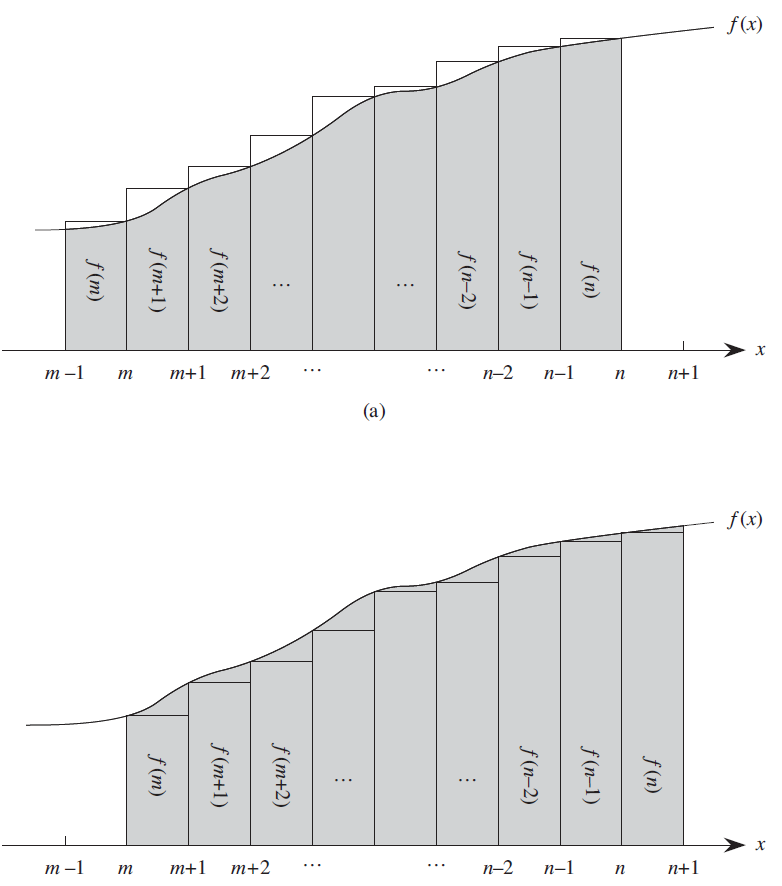
\includegraphics[scale=0.5]{./QuickSort/pic/q5.png}
    \caption{증가함수의 대소비교\cite{reference1}}
\end{figure}

증가함수 $f(k)$에 대해 다음이 성립함을 그림 4를 통해서 이해 할 수있다. 감소함수는 이와 반대로 생각하면 쉽게 해당 부등식을 이해할 수 있다.

$$\int_{m}^{n+1}f(x)dx \le \sum_{k=m}^n f(k) \le \int_{m-1}^{n}f(x)dx$$

다음 두가지 방식으로 계산한다

$\sum_{k=2}^n \dfrac{1}{k}+1 \le \int_{2}^{n+1}f(x)dx +1= \ln (x)+1 = O(\ln x)$

$\int_{1}^{n+1}f(x)dx =\ln (x+1) = \Omega(\ln x) \le \sum_{k=1}^n \dfrac{1}{k} $

따라서 $\sum_{k=1}^n \dfrac{1}{k} = \Theta(\lg n)$



\subsection{확률} Indicator random variables

\begin{align*}
    I\left\{ A \right\} =  
\begin{cases}
    1 &\mbox{( $H$ 발생)} \\
    0 &\mbox{( $\bar{H}$ 발생)}
\end{cases}    
\end{align*}


\begin{align*}
    E[X_A] &=  E[I \left\{ A \right\} ] \\
    &= 1 \times \Pr (A) + 0 \times \Pr(\bar{A}) \text{\footnotemark} \\
    &=\Pr (A)     
\end{align*}
\footnotetext{Pr은 A가 일어날 확률이다}
% https://tex.stackexchange.com/questions/21813/footnote-in-math-mode

